\documentclass{beamer}
\usetheme{Berlin}
\usecolortheme{dolphin}
\usepackage[utf8]{inputenc}
\usepackage[T1]{fontenc}
\usepackage{csvsimple}
\usepackage{graphicx}
\usepackage{verbatim}
\usepackage{sansmathaccent}
\pdfmapfile{+sansmathaccent.map}
\graphicspath{ {./img/} } % Path relative to the main .tex file 
\newcommand{\fg}[2]{%
  \begin{center}
      \includegraphics[width = #1\textwidth]{#2}%
  \end{center}
}

\title{Progetto di inferenza statistica: regressione lineare}
\author{Maria Chiara Menicucci, Alessandro Pedone,\\ Arianna Perotti, Leonardo Pascotto}
\institute{Politecnico di Milano}
\date{25 giugno 2024}





\begin{document}

\frame{\titlepage}
\begin{frame}
    \frametitle{Indice}
    \tableofcontents
\end{frame}

\section{Dati e domanda di ricerca}

\begin{frame}
\frametitle{Dataset}
    Indagine OECD PISA 2022: \\
    \texttt{https://www.oecd.org/pisa/data/2022database/}\\
    Estraiamo i dati relativi all'Italia: 
    \begin{itemize}
        \item $6920$ osservazioni %(nessun NA)
        \item $8$ covariate continue
        \item $7$ covariate categoriche
    \end{itemize}
\end{frame}

\begin{frame}
\frametitle{Domanda di ricerca}
	Vogliamo fare una regressione lineare per spiegare i risultati del test di matematica (\texttt{mate}) in termini di:
	\begin{itemize}
    \item caratteristiche personali dello studente
    \item contesto familiare
	\item impegno individuale 
	\item ambiente scolastico
	\end{itemize}
\end{frame}

\begin{frame}
    Utilità del modello:
    \begin{itemize}
        \item comprendere quali fattori influenzano il rendimento in matematica
        \item supporto a decisioni concrete che le scuole devono prendere
    \end{itemize}
\end{frame}

\begin{frame}
\frametitle{Risposta}
\fg{0.8}{histmate}
\end{frame}

\begin{frame}
    \frametitle{Covariate}
    \begin{itemize}
    \item{\makebox[2cm]{\texttt{ESCS}\hfill} : index of economic, social and cultural status}
    \item{\makebox[2cm]{\texttt{FAMSUP}\hfill} : family support}
    \item{\makebox[2cm]{\texttt{FAMSUPSL}\hfill} : family support for self-directed learning}
    \item{\makebox[2cm]{\texttt{ANXMAT}\hfill} : mathematics anxiety}
    \item{\makebox[2cm]{\texttt{SCHRISK}\hfill} : school safety risks}
    \item{\makebox[2cm]{\texttt{BULLIED}\hfill} : being bullied}
    \item{\makebox[2cm]{\texttt{TEACHSUP}\hfill} : mathematics teacher support}
    \item{\makebox[2cm]{\texttt{SMRATIO}\hfill} : student-mathematics teacher ratio}
    \end{itemize}
\end{frame}

\begin{frame}
    \begin{itemize}
    \item{\makebox[2cm]{\texttt{grade}\hfill} : prima, seconda e terza superiore}
    \item{\makebox[2cm]{\texttt{gender}\hfill} : $0$ (M), $1$ (F)}
    \item{\makebox[2cm]{\texttt{immig}\hfill} : $0$ (no) e $1$ (sì)}
    \item{\makebox[2cm]{\texttt{EXERPRAC}\hfill} : $0-10$ sessioni settimanali di attività fisica}
    \item{\makebox[2cm]{\texttt{MACTIV}\hfill} : $0-5$ attività extracurr. legate alla matematica}
    \item{\makebox[2cm]{\texttt{mathtime}\hfill} : $1-6$ studio della matematica}
    \item{\makebox[2cm]{\texttt{studytime}\hfill} : $1-6$ studio in generale}
    \end{itemize}
\end{frame}

%\begin{frame}
%\frametitle{Tempo di studio}
%La seguente legenda è valida sia per \texttt{mathtime} che per \texttt{studytime}
%\begin{enumerate}[1 :]
%\item fino a $30'$ al giorno 
%\item $30'- 1$ ora al giorno 
%\item $1-2$ ore al giorno 
%\item $2-3$ ore al giorno 
%\item $3-4$ ore al giorno 
%\item più di 4 ore al giorno
%\end{enumerate}
%\end{frame}

\begin{frame}
\frametitle{Visualizzazione delle correlazioni}
\fg{0.6}{cor.png}
\end{frame}



\begin{frame}
\frametitle{ANOVA}
Per ridurre il numero di categorie delle covariate categoriche sfruttiamo ANOVA. 
A titolo d'esempio\footnote{Si è seguito un procedimento analogo per \texttt{mathtime} e \texttt{EXERPRAC}}, concentriamoci su \texttt{studytime}:
\fg{0.6}{boxplotst.png}
\end{frame}

\begin{frame}[fragile]
\frametitle{ANOVA}
Non è opportuno usare un test ANOVA perché non è verificata la gaussianità intragruppo dei dati: 

{\scriptsize
\begin{verbatim}
> tapply(d$mate, d$study_time, function(x) shapiro.test(x)$p)
           1            2            3            4            5            6 
1.170236e-07 2.231728e-04 8.137330e-03 1.811259e-03 1.460014e-02 2.547258e-01 
\end{verbatim}
} 
\end{frame}

\begin{frame}[fragile]
\frametitle{Kruskal-Wallis}
Usiamo allora il test non parametrico di Kruskal-Wallis:
{\scriptsize
\begin{verbatim}
Kruskal-Wallis Test (alpha = 0.001) 
------------------------------------------------------------- 
  data : mate and as.factor(study_time) 

  statistic  : 138.3999 
  parameter  : 5 
  p.value    : 3.915209e-28 

  Result     : Difference is statistically significant. 
------------------------------------------------------------- 
\end{verbatim}
} 
\end{frame}

\begin{frame}[fragile]
\frametitle{Dunn}
Usiamo ora il test di Dunn con la correzione di Bonferroni:
{\tiny
\begin{verbatim}
> dunn.test(d$mate, as.factor(d$study_time), method = "bonferroni")
                           Comparison of x by group                            
                                 (Bonferroni)                                  
Col Mean-|
Row Mean |          1          2          3          4          5
---------+-------------------------------------------------------
       2 |  -8.043896
         |    0.0000*
         |
       3 |  -10.73415  -1.631907
         |    0.0000*     0.7702
         |
       4 |  -9.824431  -0.887767   0.836093
         |    0.0000*     1.0000     1.0000
         |
       5 |  -8.715361  -0.487160   1.125403   0.368950
         |    0.0000*     1.0000     1.0000     1.0000
         |
       6 |  -5.865791   1.907300   3.700865   2.953865   2.418035
         |    0.0000*     0.4236    0.0016*    0.0235*     0.1170
\end{verbatim}
}
Concludiamo che non c'è differenza significativa tra le classi da 2 a 5 e ha quindi senso raggrupparle nella stessa categoria.
\end{frame}

\section{Modello lineare}

\begin{frame}[fragile]
% effettuata un'opportuna categorizzazione per le covariate categoriche...
Generiamo il primo modello lineare per \texttt{mate}:
{\scriptsize
\begin{verbatim}
Call:
lm(formula = mate ~ ., data = d)

Residuals:
     Min       1Q   Median       3Q      Max 
-226.927  -42.596    0.921   43.919  213.392

Residual standard error: 64.05 on 6900 degrees of freedom
Multiple R-squared:  0.3741,	Adjusted R-squared:  0.3723 
F-statistic:   217 on 19 and 6900 DF,  p-value: < 2.2e-16 
\end{verbatim}
}
\end{frame}

\begin{frame}[fragile]

{\tiny
\begin{verbatim}

Coefficients:
                     Estimate Std. Error t value Pr(>|t|)    
(Intercept)         437.84550    4.78263  91.549  < 2e-16 ***
grade2^              32.19034    2.68624  11.983  < 2e-16 ***
grade3^              37.57639    4.20207   8.942  < 2e-16 ***
genderF             -28.79189    1.65279 -17.420  < 2e-16 ***
immigY               -2.31421    2.67021  -0.867  0.38615    
ESCS                 23.63258    0.94335  25.052  < 2e-16 ***
FAMSUP                1.62449    0.87919   1.848  0.06468 .  
FAMSUPSL            -16.79813    0.89940 -18.677  < 2e-16 ***
ANXMAT              -14.38726    0.76020 -18.926  < 2e-16 ***
math_timeabbastanza  -6.84174    3.26140  -2.098  0.03596 *  
math_timetanto      -32.80510    7.33830  -4.470 7.93e-06 ***
study_time1          21.01705    2.35324   8.931  < 2e-16 ***
study_time2          18.03680    3.34725   5.389 7.34e-08 ***
EXERPRACpoco         16.93088    2.25220   7.517 6.29e-14 ***
EXERPRACtanto       -13.41004    2.42980  -5.519 3.53e-08 ***
SCHRISK              -7.65098    0.97760  -7.826 5.78e-15 ***
BULLIED              -2.86359    0.90977  -3.148  0.00165 ** 
TEACHSUP             -0.58218    0.71107  -0.819  0.41297    
SMRATIO              -0.20457    0.03374  -6.063 1.41e-09 ***
MACTIV               12.58951    0.60931  20.662  < 2e-16 ***
---
Signif. codes:  0 ‘***’ 0.001 ‘**’ 0.01 ‘*’ 0.05 ‘.’ 0.1 ‘ ’ 1

\end{verbatim}
}
\end{frame}

\begin{frame}[fragile]
\frametitle{Validazione del modello}
\begin{figure}
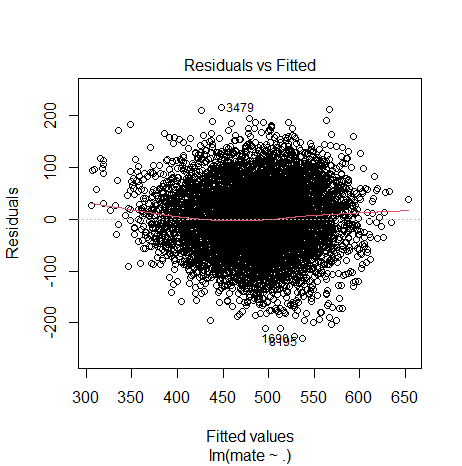
\includegraphics[width=0.475\textwidth]{omosc1}
\hfill
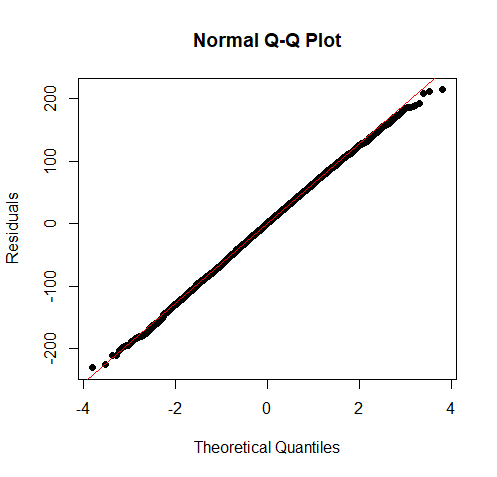
\includegraphics[width=0.475\textwidth]{norm1}
\end{figure}
{\scriptsize
\begin{verbatim}
Asymptotic one-sample Kolmogorov-Smirnov test
data:  m$residuals
D = 0.0087536, p-value = 0.664
alternative hypothesis: two-sided
\end{verbatim}
}
\end{frame}


%\section{Outliers e punti influenti}


\begin{frame}[fragile]
\frametitle{Pulizia del dataset}
Analizzando i punti influenti individuiamo 362 osservazioni, in particolare suggerite dal criterio della distanza di Cook, corrispondenti a profili di studenti molto peculiari. % cioè studenti con valori di mate eccezionalmente bassi o eccezionalmente alti, e studenti di seconda superiore con valori di mate bassi in modo anomalo rispetto a quelli di prima


% \begin{figure}
% \includegraphics[width=0.55\textwidth]{img/hist d vs d1.png}
% \end{figure}
% {\tiny
% \begin{verbatim}
% Call:
% lm(formula = mate ~ ., data = d1)

% Residuals:
%     Min      1Q  Median      3Q     Max 
% -217.06 -106.32  -53.98  124.59  270.38 

% Coefficients:
%               Estimate Std. Error t value Pr(>|t|)    
% (Intercept)   471.7818    39.3557  11.988   <2e-16 ***
% grade2^       -10.9977    19.7517  -0.557   0.5780    
% grade3^        42.3455    25.0437   1.691   0.0918 .  
% genderF       -38.7522    15.5361  -2.494   0.0131 *  
% immigY         28.0241    20.7705   1.349   0.1782    
% ...
% \end{verbatim}
% }
\end{frame}




\begin{frame}[fragile]
%\frametitle{Modello finale}
Rimuoviamo queste osservazioni e ripetiamo il fit del modello:
{\scriptsize
\begin{verbatim}
Call:
lm(formula = mate ~ ., data = dc)

Residuals:
     Min       1Q   Median       3Q      Max 
-208.732  -39.754    0.427   40.747  186.572 

Residual standard error: 57.21 on 6538 degrees of freedom
Multiple R-squared:  0.4454,	Adjusted R-squared:  0.4438 
F-statistic: 276.3 on 19 and 6538 DF,  p-value: < 2.2e-16
\end{verbatim}
}
\end{frame}

\begin{frame}[fragile]

{\tiny
\begin{verbatim}
Coefficients:
               Estimate Std. Error t value Pr(>|t|)    
(Intercept)   438.90613    4.43227  99.025  < 2e-16 ***
grade2^        34.34865    2.50746  13.699  < 2e-16 ***
grade3^        38.64076    4.05337   9.533  < 2e-16 ***
genderF       -28.48306    1.51639 -18.783  < 2e-16 ***
immigY         -4.27368    2.48070  -1.723   0.0850 .  
ESCS           24.72479    0.86930  28.442  < 2e-16 ***
FAMSUP          1.09726    0.81749   1.342   0.1796    
FAMSUPSL      -18.12601    0.84071 -21.560  < 2e-16 ***
ANXMAT        -15.90400    0.71002 -22.399  < 2e-16 ***
math_time1     -4.14156    3.09585  -1.338   0.1810    
math_time2    -33.92921    8.17806  -4.149 3.38e-05 ***
study_time1    19.80758    2.18930   9.047  < 2e-16 ***
study_time2    15.84059    3.12187   5.074 4.00e-07 ***
EXERPRACpoco   15.76601    2.08100   7.576 4.05e-14 ***
EXERPRACtanto -15.16094    2.24528  -6.752 1.58e-11 ***
SCHRISK        -7.83478    0.90879  -8.621  < 2e-16 ***
BULLIED        -1.64090    0.84658  -1.938   0.0526 .  
TEACHSUP        0.17820    0.65791   0.271   0.7865    
SMRATIO        -0.20343    0.03094  -6.576 5.21e-11 ***
MACTIV         13.18464    0.56113  23.497  < 2e-16 ***
---
Signif. codes:  0 ‘***’ 0.001 ‘**’ 0.01 ‘*’ 0.05 ‘.’ 0.1 ‘ ’ 1
\end{verbatim}
}
\end{frame}


%selezione manuale delle covariate

% \begin{frame}[fragile]
% \frametitle{Selezione del modello}
% Escludiamo ora \texttt{immig}, \texttt{TEACHSUP}, \texttt{FAMSUP} perché poco significative
% {\scriptsize
% \begin{verbatim}
% Call:
% lm(formula = mate ~ ., data = d)

% Residuals:
%      Min       1Q   Median       3Q      Max 
% -230.717  -42.366    1.109   43.876  214.159 

% Residual standard error: 64.06 on 6903 degrees of freedom
% Multiple R-squared:  0.3736,	Adjusted R-squared:  0.3722 
% F-statistic: 257.4 on 16 and 6903 DF,  p-value: < 2.2e-16
% \end{verbatim}
% }
% \end{frame}

% \begin{frame}[fragile]
% \frametitle{}
% Ripetiamo la validazione:
% {\scriptsize
% \begin{verbatim}
% 	Asymptotic one-sample Kolmogorov-Smirnov test

% data:  m$residuals
% D = 0.016447, p-value = 0.05755
% alternative hypothesis: two-sided
% \end{verbatim}
% } 
% \end{frame}

% \begin{frame}
% \frametitle{}
% \begin{figure}
% \includegraphics[width=0.55\textwidth]{img/validazione gcook.png}
% \end{figure}
% \end{frame}

\begin{frame}[fragile]

\frametitle{Selezione manuale delle covariate}
Rimuoviamo \texttt{immig}:
{\scriptsize
\begin{verbatim}
Call:
lm(formula = mate ~ ., data = dc)

Residuals:
     Min       1Q   Median       3Q      Max 
-208.632  -39.856    0.183   40.696  187.078 

Residual standard error: 57.21 on 6539 degrees of freedom
Multiple R-squared:  0.4451,	Adjusted R-squared:  0.4436 
F-statistic: 291.4 on 18 and 6539 DF,  p-value: < 2.2e-16
\end{verbatim}
}
\end{frame}

\begin{frame}[fragile]

{\tiny
\begin{verbatim}
Coefficients:
               Estimate Std. Error t value Pr(>|t|)    
(Intercept)   437.92500    4.39619  99.615  < 2e-16 ***
grade2^        35.30556    2.44553  14.437  < 2e-16 ***
grade3^        39.75482    4.00206   9.934  < 2e-16 ***
genderF       -28.53831    1.51628 -18.821  < 2e-16 ***
ESCS           25.08317    0.84418  29.713  < 2e-16 ***
FAMSUP          1.15757    0.81686   1.417   0.1565    
FAMSUPSL      -18.09845    0.84068 -21.528  < 2e-16 ***
ANXMAT        -15.95861    0.70942 -22.495  < 2e-16 ***
math_time1     -4.25476    3.09562  -1.374   0.1694    
math_time2    -34.30694    8.17635  -4.196 2.75e-05 ***
study_time1    19.65679    2.18788   8.984  < 2e-16 ***
study_time2    15.74661    3.12186   5.044 4.68e-07 ***
EXERPRACpoco   15.79103    2.08126   7.587 3.72e-14 ***
EXERPRACtanto -15.14688    2.24560  -6.745 1.66e-11 ***
SCHRISK        -7.89359    0.90828  -8.691  < 2e-16 ***
BULLIED        -1.66334    0.84660  -1.965   0.0495 *  
TEACHSUP        0.16107    0.65794   0.245   0.8066    
SMRATIO        -0.20371    0.03094  -6.584 4.93e-11 ***
MACTIV         13.12360    0.56009  23.431  < 2e-16 ***
---
Signif. codes:  0 ‘***’ 0.001 ‘**’ 0.01 ‘*’ 0.05 ‘.’ 0.1 ‘ ’ 1
\end{verbatim}
}
\end{frame}

\begin{frame}[fragile]
Rimuoviamo \texttt{FAMSUP}:
{\scriptsize
\begin{verbatim}
Call:
lm(formula = mate ~ ., data = dc)

Residuals:
     Min       1Q   Median       3Q      Max 
-207.665  -39.997    0.385   40.773  185.698 

Residual standard error: 57.22 on 6540 degrees of freedom
Multiple R-squared:  0.4449,	Adjusted R-squared:  0.4435 
F-statistic: 308.4 on 17 and 6540 DF,  p-value: < 2.2e-16
\end{verbatim}
}
\end{frame}

\begin{frame}[fragile]

{\tiny
\begin{verbatim}
Coefficients:
               Estimate Std. Error t value Pr(>|t|)    
(Intercept)   437.43138    4.38270  99.809  < 2e-16 ***
grade2^        35.40735    2.44466  14.484  < 2e-16 ***
grade3^        40.00901    3.99834  10.006  < 2e-16 ***
genderF       -28.45379    1.51522 -18.779  < 2e-16 ***
ESCS           25.13894    0.84332  29.809  < 2e-16 ***
FAMSUPSL      -17.74475    0.80284 -22.103  < 2e-16 ***
ANXMAT        -15.91695    0.70887 -22.454  < 2e-16 ***
math_time1     -4.26707    3.09585  -1.378   0.1682    
math_time2    -34.39386    8.17675  -4.206 2.63e-05 ***
study_time1    19.87020    2.18286   9.103  < 2e-16 ***
study_time2    16.07646    3.11341   5.164 2.49e-07 ***
EXERPRACpoco   15.81812    2.08134   7.600 3.38e-14 ***
EXERPRACtanto -15.04230    2.24456  -6.702 2.23e-11 ***
SCHRISK        -7.93690    0.90784  -8.743  < 2e-16 ***
BULLIED        -1.79323    0.84169  -2.131   0.0332 *  
TEACHSUP        0.23848    0.65572   0.364   0.7161    
SMRATIO        -0.20419    0.03094  -6.599 4.45e-11 ***
MACTIV         13.16073    0.55952  23.521  < 2e-16 ***
---
Signif. codes:  0 ‘***’ 0.001 ‘**’ 0.01 ‘*’ 0.05 ‘.’ 0.1 ‘ ’ 1
\end{verbatim}
}
\end{frame}

\begin{frame}[fragile]
Rimuoviamo \texttt{TEACHSUP}:
{\scriptsize
\begin{verbatim}
CCall:
lm(formula = mate ~ ., data = dc)

Residuals:
     Min       1Q   Median       3Q      Max 
-207.722  -40.002    0.245   40.710  185.655 

Residual standard error: 57.21 on 6541 degrees of freedom
Multiple R-squared:  0.4449,	Adjusted R-squared:  0.4436 
F-statistic: 327.7 on 16 and 6541 DF,  p-value: < 2.2e-16
\end{verbatim}
}
\end{frame}

\begin{frame}[fragile]

{\tiny
\begin{verbatim}
Coefficients:
               Estimate Std. Error t value Pr(>|t|)    
(Intercept)   437.39354    4.38118  99.835  < 2e-16 ***
grade2^        35.37684    2.44306  14.481  < 2e-16 ***
grade3^        40.00389    3.99805  10.006  < 2e-16 ***
genderF       -28.45443    1.51512 -18.780  < 2e-16 ***
ESCS           25.12462    0.84235  29.827  < 2e-16 ***
FAMSUPSL      -17.72026    0.79996 -22.152  < 2e-16 ***
ANXMAT        -15.95472    0.70117 -22.754  < 2e-16 ***
math_time1     -4.29282    3.09483  -1.387   0.1655    
math_time2    -34.47894    8.17286  -4.219 2.49e-05 ***
study_time1    19.91440    2.17933   9.138  < 2e-16 ***
study_time2    16.14122    3.10811   5.193 2.13e-07 ***
EXERPRACpoco   15.80951    2.08106   7.597 3.46e-14 ***
EXERPRACtanto -15.05149    2.24427  -6.707 2.16e-11 ***
SCHRISK        -7.95912    0.90572  -8.788  < 2e-16 ***
BULLIED        -1.81946    0.83854  -2.170   0.0301 *  
SMRATIO        -0.20415    0.03094  -6.599 4.48e-11 ***
MACTIV         13.15504    0.55927  23.522  < 2e-16 ***
---
Signif. codes:  0 ‘***’ 0.001 ‘**’ 0.01 ‘*’ 0.05 ‘.’ 0.1 ‘ ’ 1
\end{verbatim}
}
\end{frame}

% \begin{frame}[fragile]
% Rimuoviamo \texttt{BULLIED}:
% \end{frame}

\begin{frame}[fragile]
La forward e backward selection con il BIC %che in teoria penalizza anche più dell'AIC l'alto numero di covariate!
rimuove anche \texttt{BULLIED}:
{\tiny
\begin{verbatim}
> step(m0, direction = "both", scope=formula(m1), trace = F, k = log(n))

Call:
lm(formula = mate ~ ESCS + MACTIV + ANXMAT + FAMSUPSL + EXERPRAC + 
    gender + grade + SCHRISK + study_time + SMRATIO + math_time, 
    data = dc)

Coefficients:
  (Intercept)           ESCS         MACTIV         ANXMAT       FAMSUPSL  
     437.6584        25.0999        13.1822       -16.1007       -17.6605  
 EXERPRACpoco  EXERPRACtanto        genderF        grade2^        grade3^  
      15.9298       -14.9732       -28.4018        35.8370        40.7948  
      SCHRISK    study_time1    study_time2        SMRATIO     math_time1  
      -8.3807        20.0084        16.0899        -0.2045        -4.5003  
   math_time2  
     -35.0074  
\end{verbatim}
}
\end{frame}


% \begin{frame}[fragile]
% \frametitle{Confronto}
% Aggiungiamo il calcolo dell'AIC.
% \begin{verbatim}
% AIC value
% R^2 value
% \end{verbatim}
% Il modello migliore è... confrontando AIC  e $R^2_{adj}$
% \end{frame}

\begin{frame}[fragile]

\frametitle{Modello finale}
{\footnotesize
\begin{verbatim}
Call:
lm(formula = mate ~ ., data = dc)

Residuals:
     Min       1Q   Median       3Q      Max 
-208.527  -39.948    0.447   40.738  186.789 

Residual standard error: 57.23 on 6542 degrees of freedom
Multiple R-squared:  0.4445,	Adjusted R-squared:  0.4433 
F-statistic:   349 on 15 and 6542 DF,  p-value: < 2.2e-16
\end{verbatim}
}
\end{frame}


\begin{frame}[fragile]

{\footnotesize
\begin{verbatim}
Coefficients:
               Estimate Std. Error t value Pr(>|t|)    
(Intercept)   437.65842    4.38072  99.906  < 2e-16 ***
grade2^        35.83704    2.43453  14.720  < 2e-16 ***
grade3^        40.79485    3.98253  10.243  < 2e-16 ***
genderF       -28.40179    1.51535 -18.743  < 2e-16 ***
ESCS           25.09988    0.84251  29.792  < 2e-16 ***
FAMSUPSL      -17.66053    0.79971 -22.084  < 2e-16 ***
ANXMAT        -16.10067    0.69814 -23.062  < 2e-16 ***
math_time1     -4.50026    3.09423  -1.454    0.146    
math_time2    -35.00740    8.17154  -4.284 1.86e-05 ***
study_time1    20.00839    2.17952   9.180  < 2e-16 ***
study_time2    16.08990    3.10890   5.175 2.34e-07 ***
EXERPRACpoco   15.92976    2.08092   7.655 2.21e-14 ***
EXERPRACtanto -14.97317    2.24462  -6.671 2.75e-11 ***
SCHRISK        -8.38074    0.88488  -9.471  < 2e-16 ***
SMRATIO        -0.20447    0.03095  -6.607 4.23e-11 ***
MACTIV         13.18222    0.55929  23.570  < 2e-16 ***
\end{verbatim}
}
\end{frame}

\begin{frame}[fragile]
% da sistemare
\frametitle{Validazione del modello}
\begin{figure}
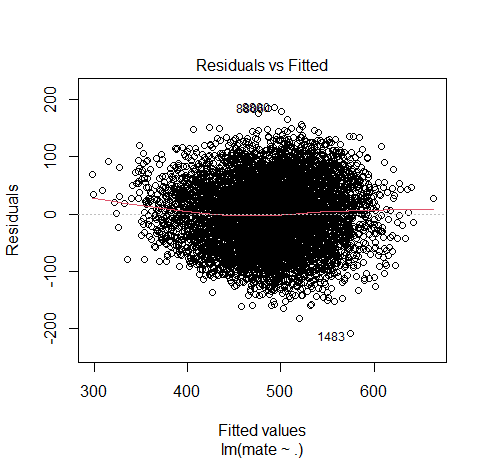
\includegraphics[width=0.475\textwidth]{omoscfinal}
\hfill
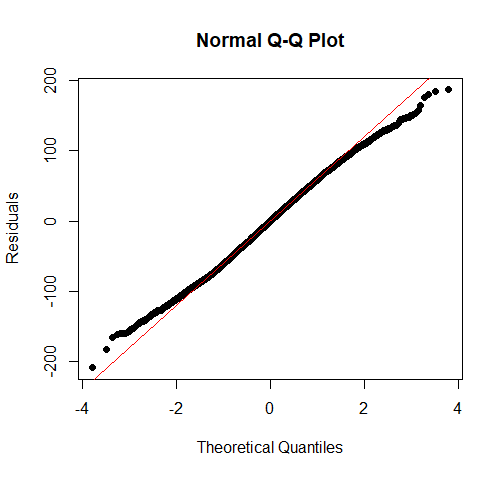
\includegraphics[width=0.475\textwidth]{normfinal}
\end{figure}
{\scriptsize
\begin{verbatim}
One-sample Kolmogorov-Smirnov test
data:  m5$residuals
D = 0.01684, p-value = 0.04849
alternative hypothesis: two-sided
\end{verbatim}
}
\end{frame}

\begin{frame}[fragile]
Calcoliamo i GVIF: non ci sono problemi di collinearità.


{\scriptsize
\begin{verbatim}
               GVIF Df GVIF^(1/(2*Df))
grade      1.060765  2        1.014857
gender     1.145016  1        1.070054
SCHRISK    1.059812  1        1.029472
ANXMAT     1.078297  1        1.038411
math_time  1.124445  2        1.029756
study_time 1.224041  2        1.051838
EXERPRAC   1.104871  2        1.025246
ESCS       1.103309  1        1.050385
FAMSUPSL   1.035756  1        1.017721
MACTIV     1.141020  1        1.068185
SMRATIO    1.065693  1        1.032324 
\end{verbatim}
}
\end{frame}

\section{Cross-validation e previsione}

\begin{frame}[fragile]
\frametitle{Cross-validation}
MSE sul traning set reale (ovvero il dataset del modello finale):
\begin{verbatim}
> mean(glm$residuals**2)
[1] 3267.384
\end{verbatim}
\end{frame}

\begin{frame}[fragile]
Facciamo la cross-validation con $10$ fold:
\begin{verbatim}
> cv.err = cv.glm(dc, glm, K = 10)
> cv.err$delta[1]
[1] 3282.943
\end{verbatim}
Miglioramento di precisione rispetto alla previsione effettuata semplicemente con la media campionaria:
\begin{verbatim}
> var(d$mate)/cv.err$delta[1]
[1] 1.990963
\end{verbatim}
\end{frame}

\begin{frame}[fragile]
Facciamo la leave-one-out cross-validation ($n=6558$ fold):
\begin{verbatim}
> cv.err = cv.glm(dc, glm, K = n)
> cv.err$delta[1]
[1] 3281.561
\end{verbatim}
Miglioramento di precisione rispetto alla previsione effettuata semplicemente con la media campionaria:
\begin{verbatim}
> var(d$mate)/cv.err$delta[1]
[1] 1.991802
\end{verbatim}
\end{frame}

\begin{frame}[fragile]
\frametitle{Intervalli di confidenza}
A titolo di esempio costruiamo degli intervalli di confidenza per il valore atteso di \texttt{mate} con $5$ osservazioni (\texttt{sample}) estratte casualmente
{\scriptsize
\begin{verbatim}
> predict(g, sample, interval = "confidence")
           fit      lwr      upr
1511  555.7920 549.9492 561.6348
2472  394.0471 386.2020 401.8922
8917  453.4244 446.9008 459.9481
2793  492.9529 487.6467 498.2590
5304  522.8707 519.3652 526.3761
\end{verbatim}
}
\end{frame}

\begin{frame}[fragile]
\frametitle{Intervalli di predizione}
A titolo di esempio costruiamo degli intervalli di predizione per \texttt{mate} con le stesse osservazioni
{\scriptsize
\begin{verbatim}
> predict(g, sample, interval = "prediction")
           fit      lwr      upr
1511  555.7920 443.4487 668.1353
2472  394.0471 281.5819 506.5123
8917  453.4244 341.0437 565.8052
2793  492.9529 380.6362 605.2695
5304  522.8707 410.6247 635.1167
\end{verbatim}
}
\end{frame}

\begin{frame}
\frametitle{Osservazioni}
\begin{itemize}
\item La stima del valore atteso è piuttosto precisa
\item La previsione del valore della variabile ha invece un'incertezza molto ampia
\item Quest'ultima si potrebbe utilizzare per identificare risultati ``improbabili'' relativi a uno studente 
\end{itemize}
\end{frame}

\end{document}